In this section we document the results for Drell-Yan background estimation using the alternative approach ($\zeta$ method) described in~\cite{ZetaNote}.
This method is inspired by ``fake-rate'' methods, in which the efficiency to pass a tight numerator cut with respect to a looser denominator cut is measured 
in a control sample enriched in background.  This fake-rate is then applied to the background dominated denominator and not numerator selection in the signal sample.  
This method is commonly used to estimate fake lepton backgrounds by extrapolating in lepton ID or isolation.  
In the $\zeta$ method the variable of interest is the MET.  
We first evaluate the efficiency to pass the signal MET cut given a loose denominator cut in a photon+jets control sample, and then apply this 
efficiency to the \dyll\ dominated dilepton events that pass the denominator cut and fail the numerator cut.

Closure tests for the $\zeta$ method with min-MET approach have already been discussed in~\cite{ZetaNote} and only the closure tests for DY MVA analysis are discussed below.
Then, the full comparison of the estimates from \routin\ and $\zeta$ method is reported.

\subsection{Closure tests for DY MVA analysis}

Tables~\ref{tab:zeta:mccloseWWzp}-\ref{tab:zeta:mccloseHWWzv} report the MC closure tests using DY MVA. 
The WP has been relaxed to reduce the statistical uncertainty.
We define ``Observed'' as the \dyll\ yield in the pass region; ``Predicted'' as the \dyll\ yield extrapolating from the fail region using the $\zeta$ method;
``Bias'' as (Predicted-Observed)/Observed.
Results suggest that a systematic uncertainty of 40\% as in the min-MET analysis is a reasonable value for DY MVA analysis as well.

\begin{table}[!hbtp]
{
 \begin{center}
 \begin{tabular}{l | c c c}
 \hline
channel       & Observed & Predicted & Bias \\
 \hline
0-jet  mm &   25.3$\pm$2.9      &   33.1$\pm$10.1     &   0.31$\pm$0.41  \\
0-jet  ee &   14.0$\pm$2.2      &   20.7$\pm$6.4      &   0.48$\pm$0.48  \\
 \hline
1-jet  mm &   25.9$\pm$2.9      &   32.5$\pm$6.3      &   0.25$\pm$0.27  \\
1-jet  ee &   15.5$\pm$2.2      &   21.2$\pm$4.0      &   0.37$\pm$0.30  \\
 \hline
\end{tabular}
\end{center}
}
\caption{MC closure: WW level, Z peak}
\label{tab:zeta:mccloseWWzp}
\end{table}

\begin{table}[!hbtp]
{
 \begin{center}
 \begin{tabular}{l | c c c}
 \hline
channel       & Observed & Predicted & Bias \\
 \hline
0-jet  mm &   11.9$\pm$2.0      &    7.7$\pm$1.5      &  -0.35$\pm$0.21  \\
0-jet  ee &    6.0$\pm$1.4      &    5.0$\pm$1.0      &  -0.16$\pm$0.28  \\
 \hline
1-jet  mm &   10.3$\pm$1.8      &   12.4$\pm$1.4      &   0.20$\pm$0.22  \\
1-jet  ee &    8.1$\pm$1.6      &    8.4$\pm$0.9      &   0.04$\pm$0.23  \\
 \hline
\end{tabular}
\end{center}
}
\caption{MC closure: HWW120 level, Z peak}
\label{tab:zeta:mccloseHWWzp}
\end{table}

\begin{table}[!hbtp]
{
 \begin{center}
 \begin{tabular}{l | c c c}
 \hline
channel       & Observed & Predicted & Bias \\
 \hline
0-jet  mm &    6.5$\pm$2.9      &    4.5$\pm$1.5      &  -0.31$\pm$0.51  \\
0-jet  ee &    2.5$\pm$0.9      &    2.2$\pm$0.7      &  -0.10$\pm$0.45  \\
 \hline
1-jet  mm &    3.0$\pm$1.0      &    3.6$\pm$0.8      &   0.20$\pm$0.44  \\
1-jet  ee &    1.4$\pm$0.6      &    1.8$\pm$0.4      &   0.30$\pm$0.54  \\
 \hline
\end{tabular}
\end{center}
}
\caption{MC closure: WW level, Z veto}
\label{tab:zeta:mccloseWWzv}
\end{table}

\begin{table}[!hbtp]
{
 \begin{center}
 \begin{tabular}{l | c c c}
 \hline
channel       & Observed & Predicted & Bias \\
 \hline
0-jet  mm &    2.6$\pm$1.8      &    1.1$\pm$0.4      &  -0.59$\pm$0.69  \\
0-jet  ee &    1.2$\pm$0.6      &    0.5$\pm$0.2      &  -0.53$\pm$0.54  \\
 \hline
1-jet  mm &    0.4$\pm$0.4      &    0.9$\pm$0.2      &   1.30$\pm$1.09  \\
1-jet  ee &    0.6$\pm$0.4      &    0.4$\pm$0.1      &  -0.22$\pm$0.75  \\
 \hline
\end{tabular}
\end{center}
}
\caption{MC closure: HWW120 level, Z veto}
\label{tab:zeta:mccloseHWWzv}
\end{table}

Comparing the DY MVA ditribution in data and in MC, especially in the 0-jet bin, a large disagreement is visible at high DY MVA values (Fig.~\ref{fig:dymva_noscale}).
This effect is caused by the underestimation of \Wjets\ background.

In a photon sample, the \Wjets\ background is due to electrons faking a photon and it is suppressed by vetoing a pixel seed matching the ECAL super cluster.
If the veto is removed, the high DY MVA region is dominated by \Wjets\ and shows good data-MC agreement (Fig.~\ref{fig:dymva_noseedveto}).
Comparing the number of events with and without pixel seed (Fig.~\ref{fig:dymva_hasseed}) we observe that: 
\begin{itemize}
\item events with a pixel seed are completely dominated by \Wjets;
\item MC predicts more events with pixel seed than we get in data. The difference in the right bin appears small in log scale but it is very large with respect to the \Wjets\ yield in the left bin.
\end{itemize}
We conclude that the veto efficiency is not correct in MC and the \Wjets\ background needs to be normalized from data.

As already mentioned, the total \Wjets\ yield without applying the pixed seed veto in data is well reproduced by MC: 
\begin{equation}
N_{Wj}(pass, data)+N_{Wj}(fail, data) = N_{Wj}(pass, MC)+N_{Wj}(fail, MC);
\end{equation}
therefore, the number or \Wjets\ events passing the pixel seed veto in data can be estimated as:
\begin{equation}
N_{Wj}(pass, data) = N_{Wj}(pass, MC)+N_{Wj}(fail, MC)-N_{Wj}(fail, data)
\label{eq:zeta:wj}
\end{equation}
where $N_{Wj}(fail, data)$ is obtained after subtracting the small non-\Wjets\ contributions obtained from MC.
Eq.~\ref{eq:zeta:wj} is used to derive data-to-MC scale factors for \Wjets\ background as a function of the photon \pt\ (Table~\ref{tab:zeta:wj_sf}).
After applying the scale factors, the DY MVA distribution (Fig.~\ref{fig:dymva_scaled}) shows a better data-MC agreement in the 0-jet bin.

%%%%%%%%
\begin{figure}[!hbtp]
\begin{center}
\subfigure[0-jet bin]{\label{subfig:dymva_noscale_0j}
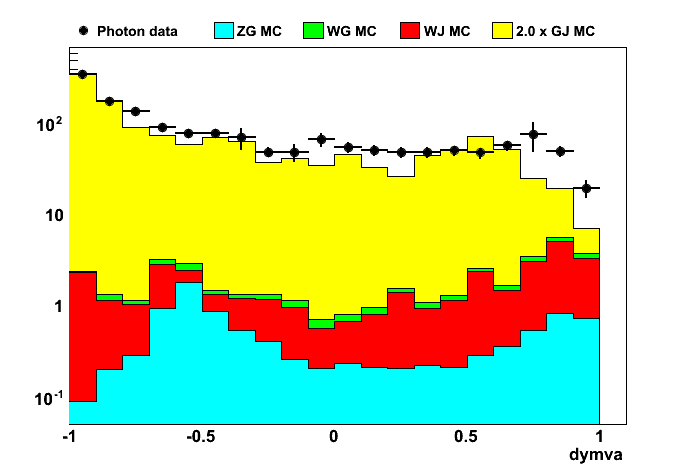
\includegraphics[width=.4\textwidth]{figures/photon_dymva_noscale_0j.png}}
\subfigure[1-jet bin]{\label{subfig:dymva_noscale_1j}
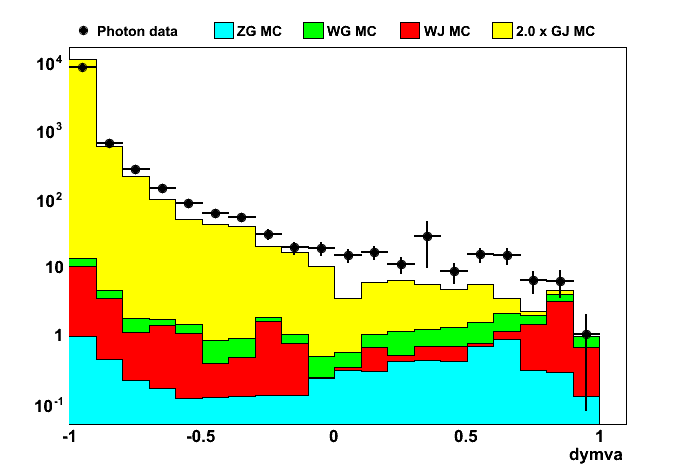
\includegraphics[width=.4\textwidth]{figures/photon_dymva_noscale_1j.png}}\\
\caption{DY MVA distribution in data and in MC after full selection in the photon dataset.
For visualization purposes, the $\gamma$+jets~ contribution from MC is scaled by a had-hoc scale factor to macth data in the bulk of the distribution.
}
\label{fig:dymva_noscale}
\end{center}
\end{figure}
%%%%%%%%

%%%%%%%%
\begin{figure}[!hbtp]
\begin{center}
\subfigure[0-jet bin]{\label{subfig:dymva_noseedveto_0j}
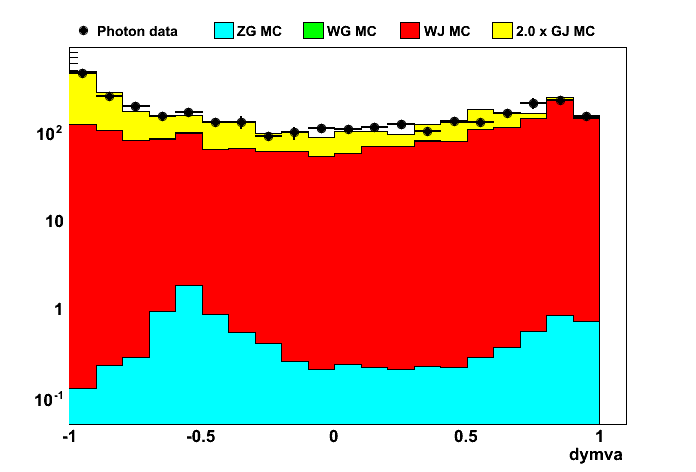
\includegraphics[width=.4\textwidth]{figures/photon_dymva_noseedveto_0j.png}}
\subfigure[1-jet bin]{\label{subfig:dymva_noseedveto_1j}
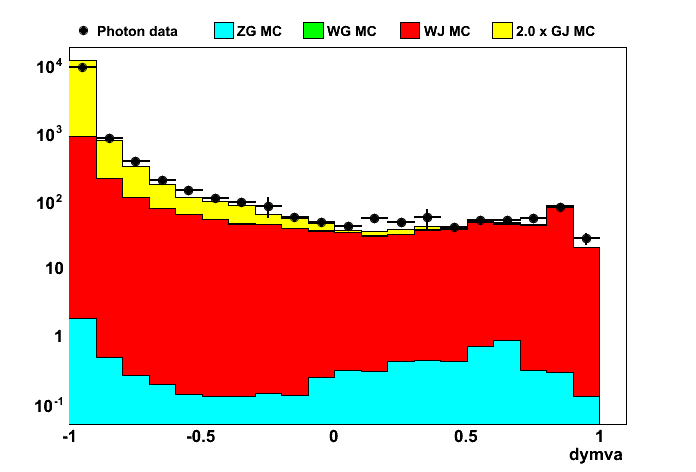
\includegraphics[width=.4\textwidth]{figures/photon_dymva_noseedveto_1j.png}}\\
\caption{DY MVA distribution in data and in MC after full selection except that the pixel seed veto is not applied.
For visualization purposes, the $\gamma$+jets~ contribution from MC is scaled by a had-hoc scale factor to macth data in the bulk of the distribution.
}
\label{fig:dymva_noseedveto}
\end{center}
\end{figure}
%%%%%%%%


%%%%%%%%
\begin{figure}[!hbtp]
\begin{center}
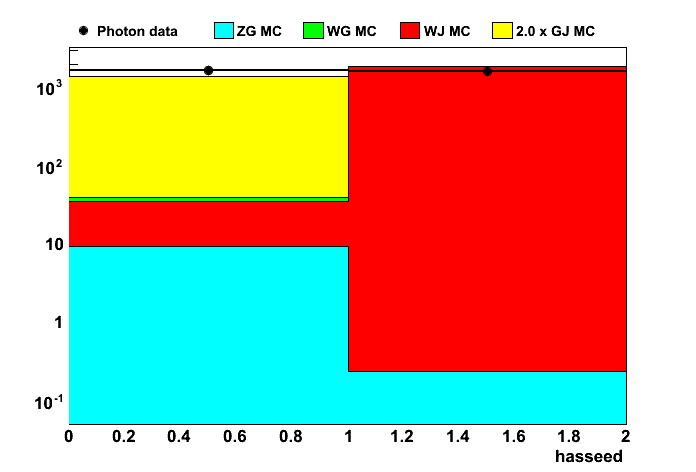
\includegraphics[width=.4\textwidth]{figures/photon_hasseed_noseedveto_0j.png}
\caption{Number of photon events in the 0-jet bin with (right bin) and without (left bin) pixel seed.
For visualization purposes, the $\gamma$+jets~ contribution from MC is scaled by a had-hoc scale factor to macth data in the bulk of the distribution.
}
\label{fig:dymva_hasseed}
\end{center}
\end{figure}
%%%%%%%%


\begin{table}[!hbtp]
{
 \begin{center}
 \begin{tabular}{l | c c }
 \hline
       & 0-jet & 1-jet \\
 \hline
45$<$\pt$(\gamma) <$50 \GeVc\ & 11.5$\pm$1.0 & -0.8$\pm$1.9 \\ 
50$<$\pt$(\gamma) <$60 \GeVc\ &  9.6$\pm$1.2 &  4.1$\pm$1.1 \\ 
\pt$(\gamma) >$60 \GeVc\      & -4.8$\pm$1.7 & -2.9$\pm$0.9 \\ 
 \hline
\end{tabular}
\end{center}
}
\caption{Scale factors for \Wjets\ background. 
Unphysical negative values are not used (no scale factor is applied in this case).
}
\label{tab:zeta:wj_sf}
\end{table}


%%%%%%%%
\begin{figure}[!hbtp]
\begin{center}
\subfigure[0-jet bin]{\label{subfig:dymva_scaled_0j}
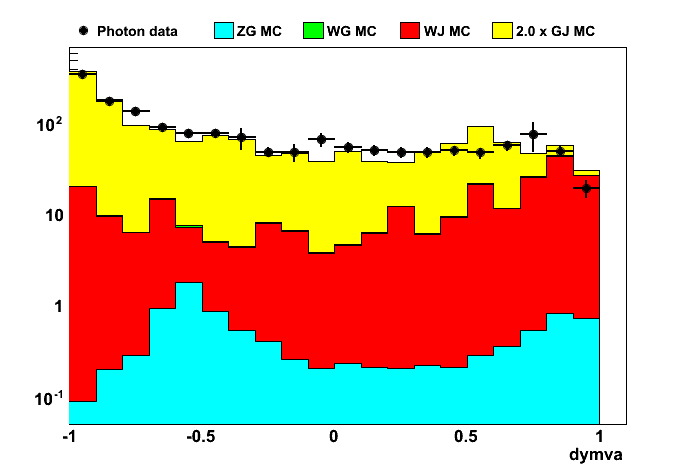
\includegraphics[width=.4\textwidth]{figures/photon_dymva_scaled_0j.png}}
\subfigure[1-jet bin]{\label{subfig:dymva_scaled_1j}
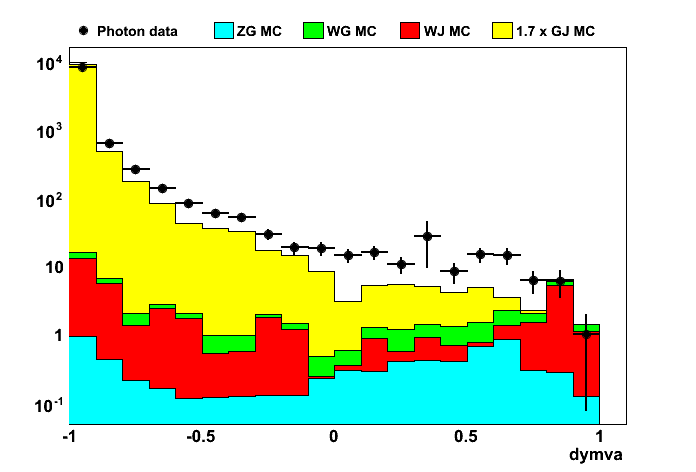
\includegraphics[width=.4\textwidth]{figures/photon_dymva_scaled_1j.png}}\\
\caption{DY MVA distribution in data and in MC after full selection in the photon dataset. 
\Wjets\ MC is scaled by the data-driven scale factors.
For visualization purposes, the $\gamma$+jets~ contribution from MC is scaled by a had-hoc scale factor to macth data in the bulk of the distribution.
}
\label{fig:dymva_scaled}
\end{center}
\end{figure}
%%%%%%%%

After subtracting the photon backgrounds, $\zeta$ values have been derived from data using the same procedure as in the min-MET case.
Closure tests have been performed in data, both at WW level and after Higgs selection (Tables~\ref{tab:zeta:datacloseWWzp}-\ref{tab:zeta:datacloseWWzv});
in the 0-jet bin, observed and predicted yields are in reasonable agreement, while in the 1-jet bin the $\zeta$ method slightly overpredicts the \dyll\ background.
However, uncertainties are large and it is hard to establish whether we have a real bias or not.

\begin{table}[!hbtp]
{
 \begin{center}
 \begin{tabular}{l | c c c}
 \hline
channel       & Observed & Predicted & Bias \\
 \hline
0-jet  mm  &  137.9$\pm$13.8  &  137.8$\pm$32.5  &   0.00$\pm$0.26    \\
0-jet  ee  &   81.7$\pm$10.5  &   85.8$\pm$20.8  &   0.05$\pm$0.29    \\
 \hline
1-jet  mm  &   31.2$\pm$9.3   &   60.9$\pm$10.7  &   0.96$\pm$0.45    \\
1-jet  ee  &   30.3$\pm$7.9   &   39.8$\pm$7.0   &   0.31$\pm$0.35    \\
 \hline
\end{tabular}
\end{center}
}
\caption{Data closure: WW level, Z peak}
\label{tab:zeta:datacloseWWzp}
\end{table}

\begin{table}[!hbtp]
{
 \begin{center}
 \begin{tabular}{l | c c c}
 \hline
channel       & Observed & Predicted & Bias \\
 \hline
0-jet  mm &   58.8$\pm$9.1   &   53.4$\pm$10.1  &  -0.09$\pm$0.23    \\
0-jet  ee &   21.7$\pm$5.9   &   33.7$\pm$6.7   &   0.55$\pm$0.41    \\
 \hline
1-jet  mm &   15.7$\pm$4.4   &   36.7$\pm$8.3   &   1.34$\pm$0.54    \\
1-jet  ee &   13.1$\pm$3.9   &   23.4$\pm$4.7   &   0.79$\pm$0.47    \\
 \hline
\end{tabular}
\end{center}
}
\caption{Data closure: HWW120 level, Z peak}
\label{tab:zeta:datacloseHWWzp}
\end{table}

\begin{table}[!hbtp]
{
 \begin{center}
 \begin{tabular}{l | c c c}
 \hline
channel       & Observed & Predicted & Bias \\
 \hline
0-jet  mm &   54.9$\pm$19.8   &   36.4$\pm$9.0    &  -0.34$\pm$0.40     \\
0-jet  ee &    2.0$\pm$13.1   &   16.1$\pm$3.9    &   7.20$\pm$6.93     \\
 \hline
1-jet  mm &    6.9$\pm$17.3   &   14.6$\pm$3.3    &   1.12$\pm$2.55     \\
1-jet  ee &   -4.8$\pm$11.9   &    8.0$\pm$1.4    &   -     \\
 \hline
\end{tabular}
\end{center}
}
\caption{Data closure: WW level, Z veto}
\label{tab:zeta:datacloseWWzv}
\end{table}


\subsection{Comparison with \routin\ results}

The Drell-Yan estimation for cut-based analysis with 5.1~\ifb data as predicted by the \routin\ (Sec.~\ref{sec:bkg_dy}) and $\zeta$ methods are 
compared in Tables~\ref{tab:zeta:routin-0j}-\ref{tab:zeta:routin-2j}.
%In the 0- and 2-jet bins the two methods provide compatible estimates, while in the 1-jet bin the $\zeta$ method predicts systematically larger yields for
%the mass points where DY MVA is used (\mHi$\leq$140 \GeVcc); this overestimation is expected from the closure tests discussed above.
In all cases, estimates from the two methods are consitent within the uncertainties.

In summary, we consider the Drell-Yan estimation used in the analysis as cross-checked with the $\zeta$ method.

\begin{table}[!hbtp]
{%\tiny
 \begin{center}
 \begin{tabular}{c | c c }
 \hline
 $m_H$ [\GeVcc] & $R_{out/in}$ & $\zeta$ \\
 \hline
     WW & 96.0$\pm$12.0 &  116.8$\pm$47.6  \\
    115 & 24.6$\pm$5.5  &   27.9$\pm$12.4  \\
    120 & 27.7$\pm$6.2  &   28.7$\pm$12.7  \\
    125 & 34.7$\pm$12.5 &   30.7$\pm$13.6  \\
    130 & 38.0$\pm$15.8 &   31.0$\pm$13.7  \\
    140 & 32.1$\pm$15.4 &   24.6$\pm$10.8  \\
    145 & 46.6$\pm$20.9 &   47.2$\pm$19.4  \\
    150 & 12.7$\pm$8.8  &   19.1$\pm$8.0   \\
    160 &  9.1$\pm$13.4 &   12.1$\pm$5.4   \\
    170 &  2.8$\pm$11.5 &    9.3$\pm$4.9   \\
    180 &  1.7$\pm$6.6  &    4.2$\pm$2.8   \\
    190 &  5.2$\pm$5.1  &    7.5$\pm$4.3   \\
    200 &  6.5$\pm$4.3  &    7.8$\pm$4.6   \\
    250 &  3.5$\pm$3.4  &   15.4$\pm$8.3   \\
    300 &  4.0$\pm$2.1  &    0.0$\pm$31.4  \\
 \hline
\end{tabular}
\end{center}
}
\caption{Comparison of \dyll\ estimates from \routin\ and $\zeta$ methods with 5.1~\ifb: 0-jet bin}
\label{tab:zeta:routin-0j}
\end{table}

\begin{table}[!hbtp]
{
 \begin{center}
 \begin{tabular}{c | c c }
 \hline
 $m_H$ [\GeVcc] & $R_{out/in}$ & $\zeta$ \\
 \hline
     WW & 120.7$\pm$26.9&  102.6$\pm$41.2  \\
    115 &  6.4$\pm$3.9  &   10.8$\pm$4.5   \\
    120 & 10.0$\pm$6.0  &   11.4$\pm$4.8   \\
    125 &  7.4$\pm$4.8  &   12.1$\pm$5.1   \\
    130 &  7.7$\pm$5.4  &   12.5$\pm$5.2   \\
    140 &  5.8$\pm$4.4  &   10.5$\pm$4.4   \\
    145 & 31.9$\pm$15.0 &   35.0$\pm$14.1  \\
    150 & 25.3$\pm$13.7 &   22.8$\pm$9.2   \\
    160 & 27.0$\pm$10.7 &   24.7$\pm$10.1  \\
    170 & 23.9$\pm$10.5 &   25.0$\pm$10.7  \\
    180 & 23.2$\pm$9.6  &   29.1$\pm$13.1  \\
    190 & 32.3$\pm$14.2 &   30.4$\pm$13.7  \\
    200 & 30.4$\pm$11.9 &   32.3$\pm$14.4  \\
    250 & 20.8$\pm$4.7  &   34.0$\pm$15.0  \\
    300 & 14.6$\pm$11.3 &   21.4$\pm$11.0  \\
 \hline
\end{tabular}
\end{center}
}
\caption{Comparison of \dyll\ estimates from \routin\ and $\zeta$ methods with 5.1~\ifb: 1-jet bin}
\label{tab:zeta:routin-1j}
\end{table}

\begin{table}[!hbtp]
{
 \begin{center}
 \begin{tabular}{c | c c }
 \hline
 $m_H$ [\GeVcc] & $R_{out/in}$ & $\zeta$ \\
 \hline
     WW &  5.5$\pm$4.6  &    5.0$\pm$2.4   \\
    115 &  2.5$\pm$2.2  &    2.6$\pm$1.3   \\
    120 &  2.5$\pm$2.1  &    3.3$\pm$1.7   \\
    125 &  2.7$\pm$2.3  &    3.4$\pm$1.7   \\
    130 &  3.8$\pm$3.2  &    3.6$\pm$1.8   \\
    140 &  4.6$\pm$3.9  &    3.8$\pm$1.9   \\
    145 &  4.6$\pm$3.9  &    3.8$\pm$1.9   \\
    150 &  4.6$\pm$3.9  &    4.2$\pm$2.0   \\
    160 &  4.8$\pm$4.1  &   10.2$\pm$5.0   \\
    170 &  5.1$\pm$4.3  &    7.4$\pm$7.9   \\
    180 &  5.3$\pm$4.5  &   35.2$\pm$24.9  \\
    190 &  5.8$\pm$4.9  &   35.2$\pm$24.9  \\
    200 &  6.3$\pm$5.3  &   35.4$\pm$25.0  \\
    250 &  5.4$\pm$4.5  &   34.1$\pm$24.9  \\
    300 &  5.4$\pm$4.5  &   34.1$\pm$25.1  \\
 \hline
\end{tabular}
\end{center}
}
\caption{Comparison of \dyll\ estimates from \routin\ and $\zeta$ methods with 5.1~\ifb: 2-jet bin}
\label{tab:zeta:routin-2j}
\end{table}

